% -*- root: main.tex -*-
Thus far, we have seen that our NLP-based approach can perform well in classifying \SATD. However, there are some observations that warrant further investigation. For example, when it comes to the different types of \SATD, we find that requirement debt tends to require less training data, which is another interesting point that is worth further investigation (Section~\ref{sec:textual_similarity}). 

\revised{Moreover, we think that is also interesting to know the performance of our approach when trained to distinguish between \SATD and non-\SATD, i.e., without using fine-grained classes of debt, such as design and requirement debt (Section~\ref{sec:coarse-grained_classes}).}{R2-9} 

Also, when performing our classification, there are several different classifiers that can be used in the Stanford Classifier toolkit, hence we investigate what is the impact of using different classifiers on the accuracy (Section~\ref{sec:underlying_classifier}).

\revised{Lastly, we analyze the overlap between the files that contain \SATD and the files that contain code smells. This is an interesting point of discussion to provide insights on how technical debt found in comments relates to code smells found by static analysis tools (Section~\ref{sec:overlap_with_static_analysis_tools}).}{R2-3}

\subsection{Textual Similarity for Design and Requirement Debt}
\label{sec:textual_similarity}
For RQ3, we hypothesize that one of the reasons that the detection of requirement \SATD comments needs less training data is because such comments are more similar to each other compared to design \SATD comments. Therefore, we compare the intra-similarity of the requirement and design debt comments.

We start by calculating the term frequency-inverse document frequency (\textit{tf-idf}) weight of each design and requirement \SATD comment. Term frequency (\textit{tf}) is the simple count of occurrences that a term (i.e., word) has in a document (i.e., comment). Inverse document frequency (\textit{idf}) takes into account the number of documents that the term appears. However, as the name implies, the more one term is repeated across multiple documents the less relevant it is. Therefore, let \textit{N} be the total number of documents in a collection, the \textit{idf} of a term \textit{t} is defined as follows: \(idf_{t} = log\frac{N}{df_{t}}\). The total \textit{tf-idf} weight of a document is equal to the sum of each individual term \textit{tf-idf} weight in the document. Each document is represented by a \textit{document vector} in a \textit{vector space model}. 

Once we have the \textit{tf-idf} weights for the comments, we calculate the \textit{cosine similarity} between the comments. The Cosine similarity can be viewed as the \textit{dot product} of the normalized versions of two document vectors (i.e., two comments)~\cite{Manning2008book}. The value of the cosine distance ranges between 0 to 1, where 0 means that the comments are not similar at all and 1 means that the comments are identical.

For example, the requirement \SATD dataset contains 757 comments, for which we generate a 757$\times$757 matrix (since we compare each comment to all other comments).
Finally, we take the average cosine similarity for design and requirement debt comments, respectively, and plot their distributions in Figure~\ref{fig:textual_similarity}.
Figure~\ref{fig:textual_similarity} shows that the median and the upper quartile for requirement \SATD comments are higher than the median and upper quartile for design \SATD.
The median for requirement debt comments is 0.018, whereas, the median for design debt comments is 0.011.
To ensure that the difference is statistically significant, we perform the Wilcoxon test to calculate the p-value. The calculated p-value is less than 2.2e-16 showing that the result is indeed statistically significant (i.e., p \textless 0.001). Considering our findings, our hypothesis is validated, showing that requirement \SATD comments are more similar to each other compared to design \SATD comments. This may help explain why requirement debt needs a smaller set of positive weight textual features to be detected.

\begin{figure}[t]
  \centering
  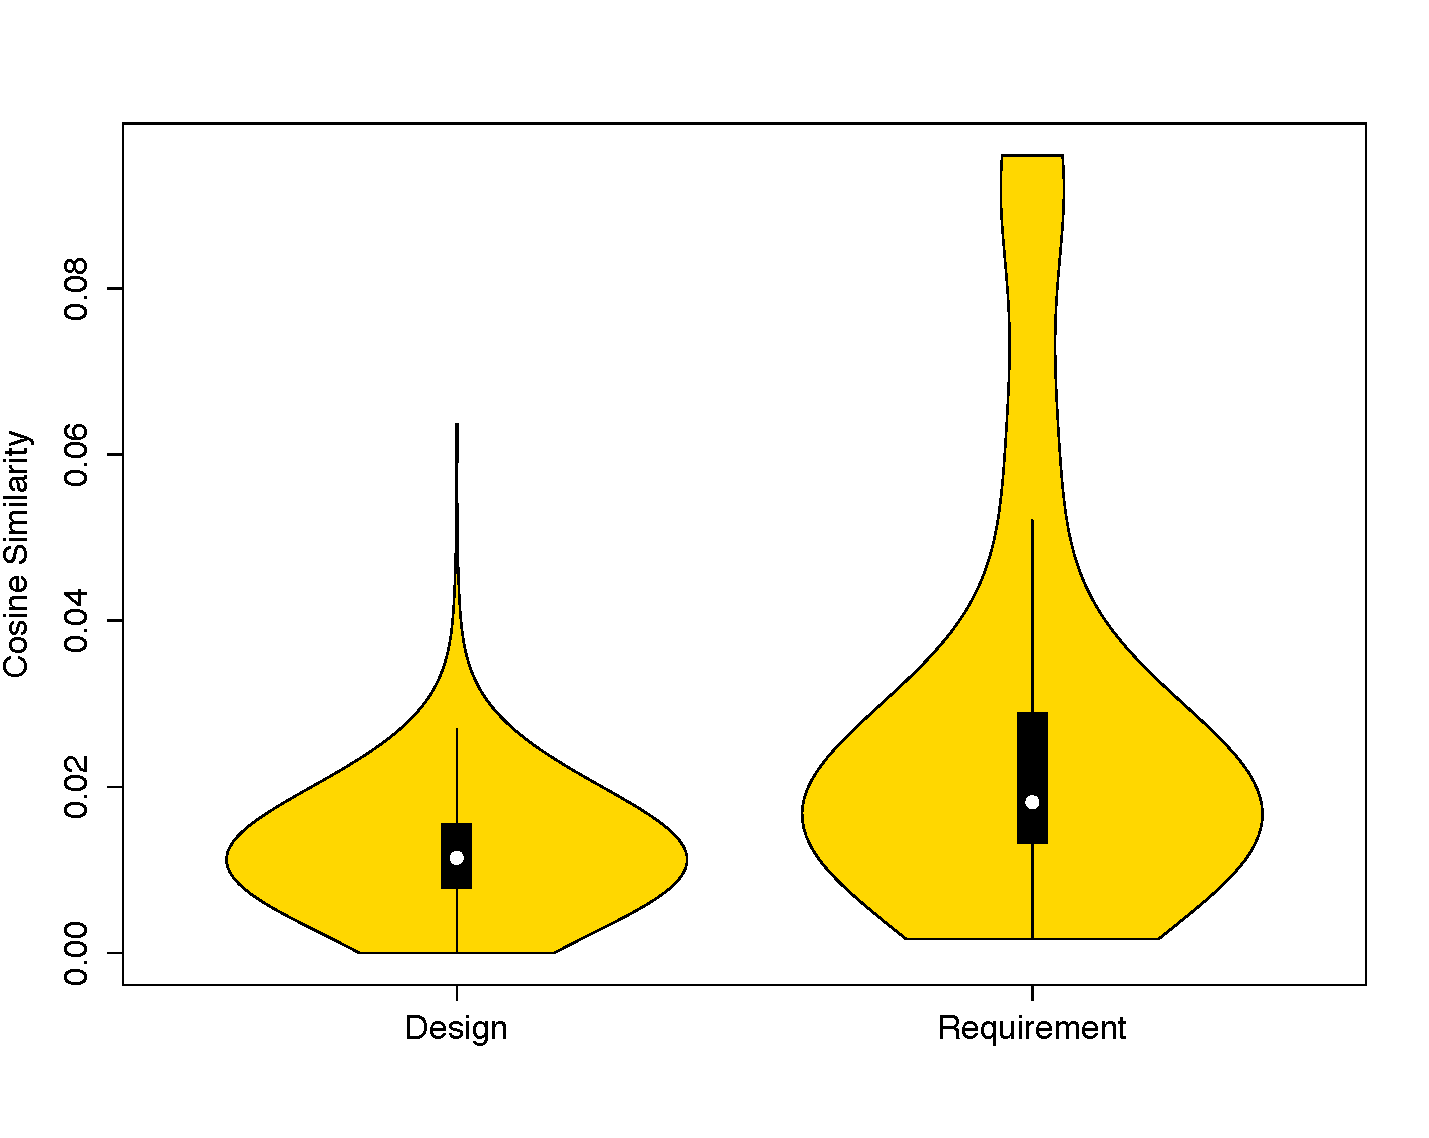
\includegraphics[width = 0.48\textwidth]{figures/textual_similarity_removing_stop_words.pdf}
  \vspace{-3mm}
  \caption{Textual Similarity Between Design and Requirement Debt Comments}
  \label{fig:textual_similarity}
\end{figure}

\revised{
\subsection{Distinguishing Self-Admitted Technical Debt from Non-Self-Admitted Technical Debt Comments}
\label{sec:coarse-grained_classes}
So far, we analyzed the performance of our NLP-based approach to identify distinct types of \SATD (i.e., design and requirement debt). However, a simpler distinction between \SATD and non-debt comments can also be interesting in the case those fine-grained classes of debt are not considered necessary by a user of the proposed NLP-based detection approach. Another reason justifying such a coarse-grained distinction is that the cost of building a training dataset with fine-grained classes of debt is more expensive, mentally challenging, and subjective than building a training dataset with just two classes (i.e., comments with and without technical debt).

In order to compute the performance of our NLP-based approach using only two classes (i.e., comments with and without technical debt), we repeat RQ1 and RQ2 with modified training and test datasets.
First, we take all design and requirement \SATD comments and label them with a common class i.e., technical debt, and the remaining comments we kept them labeled as without technical debt.
Second, we run the maximum entropy classifier in the same leave-one-out cross-project validation fashion, using the comments of 9 projects to train the classifier and the comments from the remaining project to test the classifier. We repeat this process for each of the ten projects and compute the average F1-measure. Lastly, we analyze the textual features used to identify the self-admitted technical debt comments.

Table \ref{tbl:nlpbased_performance_comparison} compares the F1-measure achieved when detecting design debt, requirement debt, separately and when detecting both combined in a single class. As we can see, the performance when detecting technical debt is very similar with the performance of the classifier when detecting design debt. This is expected, as the majority of technical debt comments in the training dataset are labeled with the design debt class. Nevertheless, the performance achieved when detecting design debt was surpassed in the projects where the classifier performed well in detecting requirement debt, for example, in Columba (0.601 vs. 0.750) and SQuirrel SQL (0.540 vs. 0.593). 

We find that the average performance when detecting design and requirement \SATD combined is better (0.636) than the performance achieved when detecting them individually (0.620 and 0.403 for design and requirement debt, respectively).

 % In addition, Table \todo{} provide precision, recall and F1-measure for each one of the projects.

\begin{table}[!thb]
  \begin{center}
    \caption{NLP-based F1-measure Performance Considering Different Types of Self-admitted Technical Debt}
    \label{tbl:nlpbased_performance_comparison}
    \begin{tabular}{l| c c c}
        \toprule
        \textbf{\thead{Project}} & \textbf{\thead{Design\\debt}} & \textbf{\thead{Requirement\\debt}} & \textbf{\thead{Technical\\debt}} \\
        \midrule
        \textbf{Ant}           & 0.517 & 0.154 & 0.512 \\
        \textbf{ArgoUML}       & 0.814 & 0.595 & 0.819 \\
        \textbf{Columba}       & 0.601 & 0.804 & 0.750 \\
        \textbf{EMF}           & 0.470 & 0.381 & 0.462 \\
        \textbf{Hibernate}     & 0.744 & 0.476 & 0.763 \\
        \textbf{JEdit}         & 0.509 & 0.091 & 0.461 \\
        \textbf{JFreeChart}    & 0.492 & 0.321 & 0.513 \\
        \textbf{JMeter}        & 0.731 & 0.237 & 0.715 \\
        \textbf{JRuby}         & 0.783 & 0.435 & 0.773 \\
        \textbf{SQuirrel}      & 0.540 & 0.541 & 0.593 \\
        \midrule 
        \textbf{Average}       & 0.620 & 0.403 & 0.636 \\ 
        \bottomrule
    \end{tabular}
  \end{center}    
\end{table}

\begin{table}[!thb]
    \begin{center}
        \caption{Top Ten Textual Features Used to Identify Different Types Self-Admitted Technical Debt}
        \label{tbl:top_ten_features_td_vs_non_td}
        \begin{tabular}{l| l l l }
        \toprule
        \textbf{\thead{Project}} & \textbf{\thead{Design\\debt}} & \textbf{\thead{Requirement\\debt}} & \textbf{\thead{Technical\\debt}} \\
        \midrule
         \textbf{1}  & hack       &   todo            & hack         \\
         \textbf{2}  & workaround &   needed          & workaround   \\
         \textbf{3}  & yuck!      &   implementation  & yuck!        \\
         \textbf{4}  & kludge     &   fixme           & kludge       \\
         \textbf{5}  & stupidity  &   xxx             & stupidity    \\
         \textbf{6}  & needed?    &   ends?           & needed?      \\
         \textbf{7}  & columns?   &   convention      & unused?      \\
         \textbf{8}  & unused?    &   configurable    & fixme        \\
         \textbf{9}  & wtf?       &   apparently      & todo         \\
         \textbf{10} & todo       &   fudging         & wtf?         \\
        \bottomrule
        \end{tabular}
    \end{center}    
\end{table}

Table \ref{tbl:top_ten_features_td_vs_non_td} shows a comparison of the top-10 textual features used to detect design and requirement debt comments separately, and those used to detect both types of debt combined in a single class.
When analyzing the top-10 textual features used to classify \SATD, we find once more, a strong overlap with the top-10 textual features used to classify design debt. The weight of the features is attributed in accordance to the frequency that each word is found in the training dataset, and therefore, the top-10 features tend to be similar with the top-10 design debt features, since design debt comments represent the majority of \SATD comments in the dataset. 

}{R2-9}

\begin{figure*}[!thb]
  \centering
  \subfigure[Design Debt]{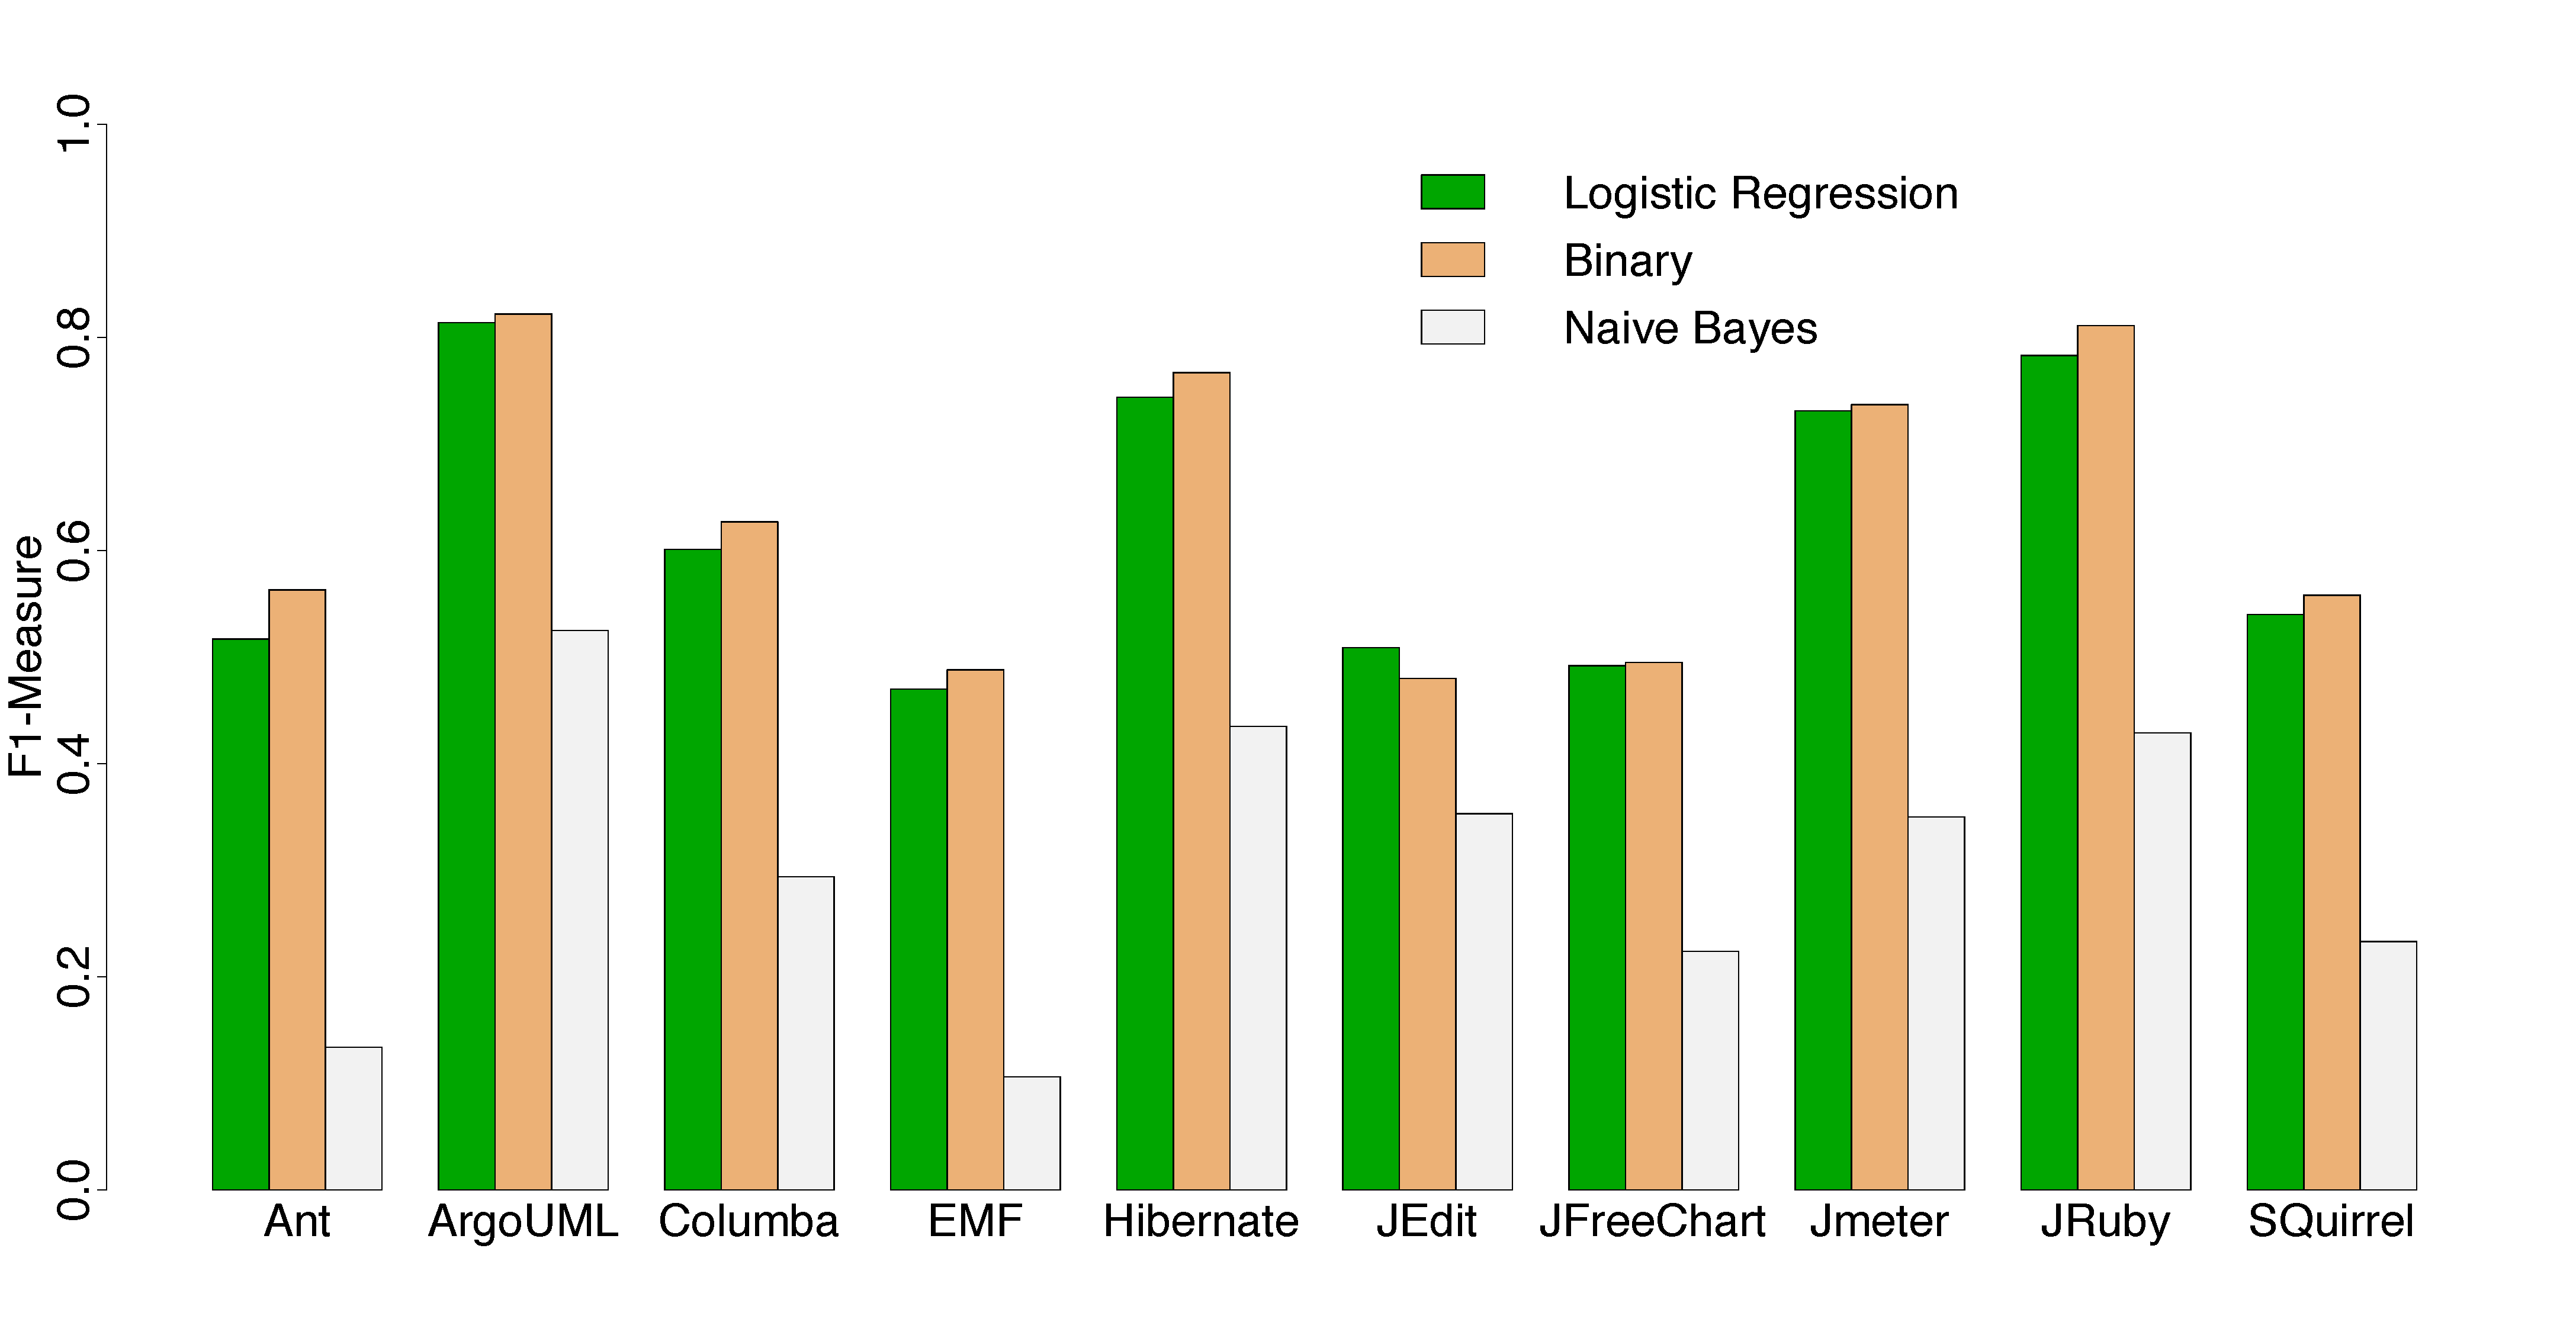
\includegraphics[width=0.48\textwidth]{figures/classifier_algorithms_comparison_design_1.pdf}
  \label{fig:algorithms_comparison_design}}
  \subfigure[Requirement Debt]{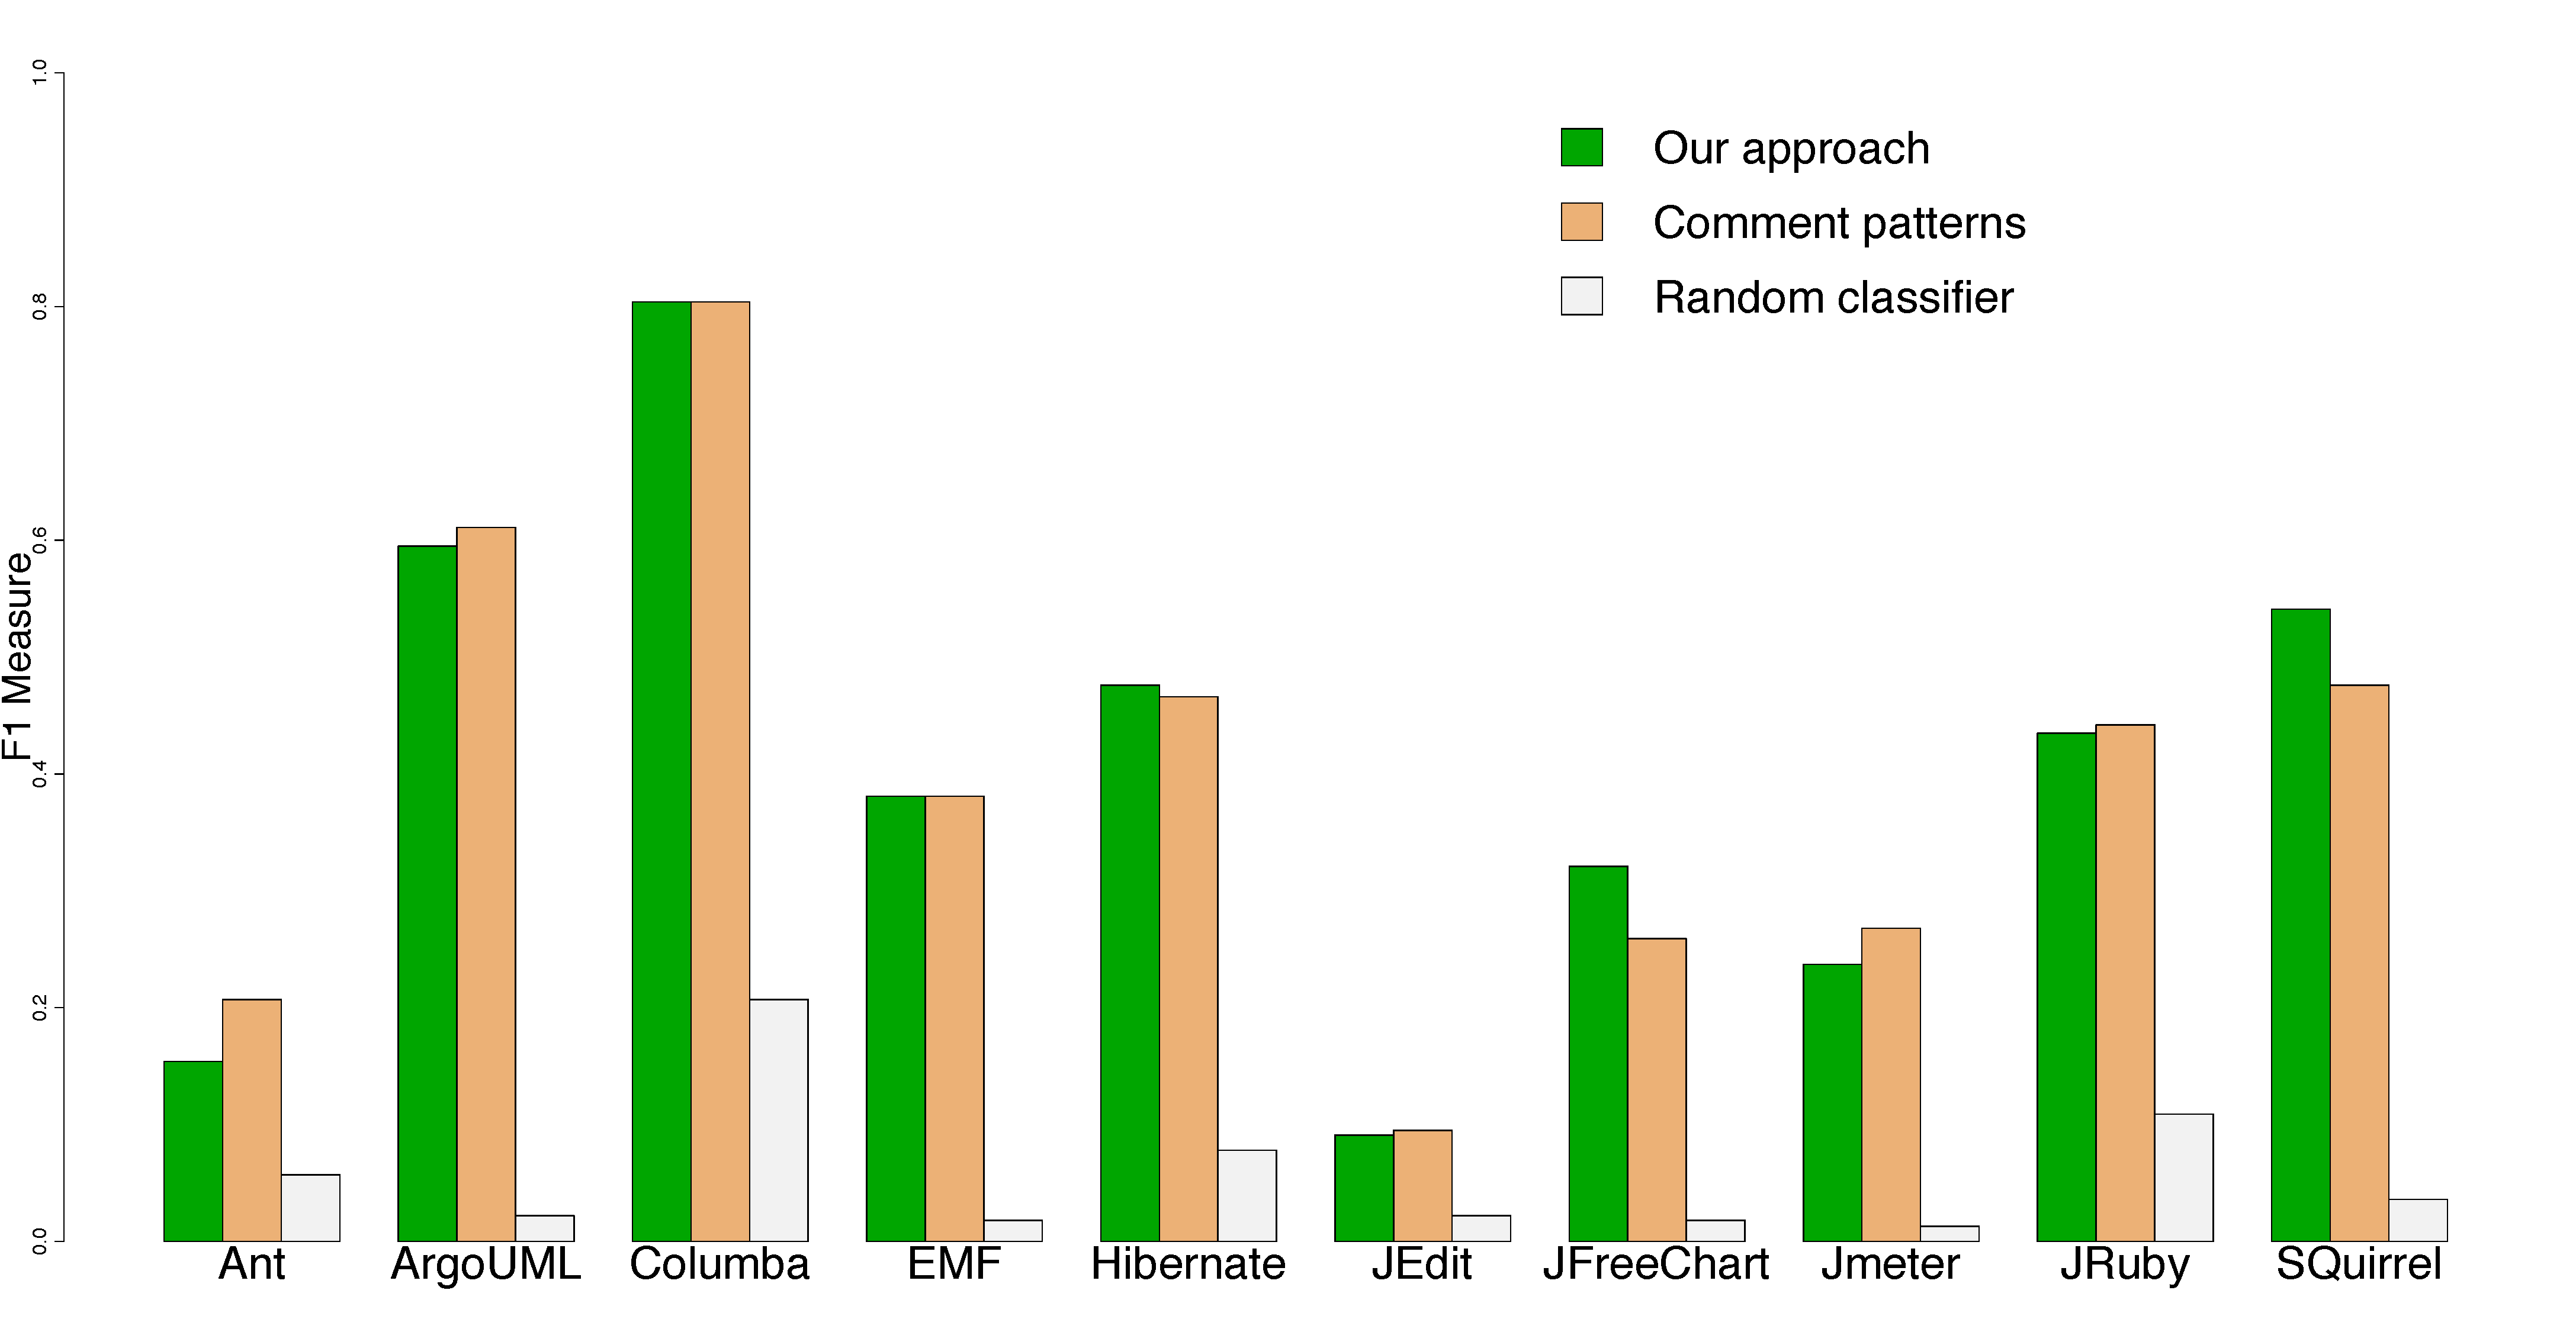
\includegraphics[width=0.48\textwidth]{figures/classifier_algorithms_comparison_implementation_1.pdf}
  \label{fig:algorithms_comparison_requirement}}
  \caption{Underlying Classifier Algorithms Performance Comparison}
  \label{fig:algorithms_comparison}
\end{figure*}

\subsection{Investigating the Impact of the Underlying Classifier of the NLP Classification}
\label{sec:underlying_classifier}
In our work, all the classification done by the Stanford Classifier used a Logistic Regression classifier. However, the Stanford Classifier can use other classifiers. In order to examine the impact of the underlying classifier on our results, we chose the other two algorithms to execute the classification with, namely the Naive Bayes generative classifier and the Binary classifier.
 
Figures \ref{fig:algorithms_comparison_design} and \ref{fig:algorithms_comparison_requirement} compare the performance between the three different algorithms. We find that Naive Bayes has the worst average F1-measure of 0.30 and 0.05 for design and requirement technical debt, respectively. Based on our findings, the Naive Bayes algorithm favors recall at the expense of precision. For example, while classifying design debt, the average recall was of 0.84 and precision 0.19. The two other algorithms present more balanced results compared to Naive Bayes, and the difference in performance between them is not as accentuate. The Logistic Regression classifier achieved F1-measures of 0.62 and 0.40, while the binary classifier F1-measures were 0.63 and 0.40, for design and requirement \SATD, respectively. Tables \ref{tbl:improvement_f1measure_between_classifiers_design} and \ref{tbl:improvement_f1measure_between_classifiers_requirement} in the Appendix section provide detailed data for each compared algorithm for all ten projects.

Although the Binary classification has a slightly better performance, for our purpose, the Logistical Regression algorithm provide more insightful features. These features were analyzed and presented in RQ2. 

\revised{According to previous work, developers hate to deal with false positives results (i.e., low precision) \cite{Bessey2010FBL,Ernst2015FSE,Sadowski2015ICSE}. Due to this fact, we choose to present our results in this study using the Logistical Regression algorithm, which has an average precision of 0.716 throughout all projects. However, results that favors recall over precision (e.g. Naives Bayes algorithm) might well be fine if a manual process to filter out false positives is in place, as reported by Berry et al. \cite{Berry2012book}. }{R2-6}

\revised{One important question to ask when choosing what kind of classifier to use is how much training data is currently available. Must often, the trickiest part of applying a machine learning classifier in real world applications is creating or obtaining enough training data. If you have fairly little data at your disposal, and you are going to train a supervised classifier then machine learn theory recommends classifiers with high bias, such as Naive Bayes~\cite{Forman2004PKDD,Ng2001NIPS}. If there is a reasonable amount of labeled data, then you are in good stand to use most kinds of classifiers~\cite{Manning2008book}. For instance, you may wish to use an Support Vector Machine (SVM), a decision tree or, like in our study, a max entropy classifier. If a huge amount of data is available, then the choice of classifier probably has little effect on your results and the best choice may be unclear~\cite{Banko2001book}. It may be best to choose a classifier based on the scalability of training or even runtime efficiency.}{R2-11}

\revised{
\subsection{Investigating the Overlap Between Technical Debt Found in Comments and Technical Debt Found by Static Analysis Tools}
\label{sec:overlap_with_static_analysis_tools}
Thus far, we analyzed technical debt that was expressed by developers through source code comments. However, there are other ways to identify technical debt, such as architectural reviews, documentation analysis, and static analysis tools. To date, using static analysis tools is the most established approach to identify technical debt in the source code. In general, static analysis tools parse the source code of a project to calculate metrics and identify possible object oriented design violations, also known as code smells, anti-patterns, or design technical debt, based on some fixed metric threshold values. 

In this subsection, we analyze the overlap between what our NLP-based approach identifies as technical debt and what a static analysis tool identifies as technical debt.
We selected JDeodorant as the static analysis tool, since it supports the detection of three popular code smells, namely Long Method, God Class, and Feature Envy.
We avoided the use of metric-based code smell detection tools, because they tend to have high false positive rates and flag a large portion of the code base as problematic~\cite{Fontana:2016}.
On the other hand, JDeodorant detects only \textit{actionable} code smells (i.e., code smells for which a behavior-preserving refactoring can be applied to resolve them),
and does not rely on any metric thresholds, but rather applies static source code analysis to detect structural anomalies and suggest refactoring opportunities to eliminate them.

First, we analyzed our 10 open source projects using JDeodorant. The result of this analysis is a list of Java files that were identified having at least one instance of
the Long Method, God Class, and Feature Envy code smells. These code smells have been extensively investigated in the literature, and are considered to occur frequently~\cite{Olbrich:2010, Sjoberg:2013}.
Second, we created a similar list containing the files that were identified with \SATD comments. Finally, we examined the overlap of the two lists of files.
It should be emphasized that we did not examine if the \SATD comments actually discuss the detected code smells, but only if there is a co-occurrence at file-level.

Table \ref{tbl:static_analysis_tool_and_self_admitted_technical_debt_overlap_using_jdeodorant} provides details about each of the projects used in our study. The columns of Table \ref{tbl:static_analysis_tool_and_self_admitted_technical_debt_overlap_using_jdeodorant} present the total number of files with \SATD, followed by the number of files containing \SATD comments and at least one code smell instance,
along with the percentage over the total number of files with \SATD, for Long Method, Feature Envy, God Class, and all combined code smells, respectively. 

JMeter, for example, has 200 files that contain \SATD comments, and 143 of these files also contain at least one Long Method code smell (i.e., 71.5\%). In addition, we can see that 20.5\% of the files that have \SATD are involved in Feature Envy code smells, and 48.5\% of them are involved in God Class code smells. In summary, we see that 80.5\% of the files that contain \SATD comments are also involved in at least one of the three examined code smells.     

We find that the code smell that overlaps the most with \SATD is Long Method. Intuitively, this is expected, since Long Method is a common code smell and may have multiple instances per file, because it is computed at method level.
The overlap between files with \SATD and Long Method ranged from 43.6\% to 82\% of all the files containing \SATD comments, and considering all projects, the average overlap is 65\%. In addition, 44.2\% of the files with \SATD comments are also involved in God Class code smells, and 20.7\% in Feature Envy code smells. Taking all examined code smells in consideration we find that, on average, 69.7\% of files containing \SATD are also involved in at least one of the three examined code smells. 

\begin{table*}[!thb]
    \begin{center}
        \caption{Static Analysis Tool and Self-admitted Technical Debt Overlap (Using JDeodorant)}
        \label{tbl:static_analysis_tool_and_self_admitted_technical_debt_overlap_using_jdeodorant}
        \begin{tabular}{l| c c c c c c c c c}
        \toprule
        \textbf{\thead{Project}} & \textbf{\thead{\# of \\files with\\ SATD }} & \textbf{\thead{\# of SATD \\files with \\ Long \\Method }} & \textbf{\thead{\%  of SATD \\files with \\ Long \\Method}} & \textbf{\thead{\# of SATD \\files with \\ Feature \\Envy}} & \textbf{\thead{\% of SATD \\files with \\ Feature \\Envy}} & \textbf{\thead{\# of SATD\\ files with \\ God \\Class}} & \textbf{\thead{\% of SATD\\ files with \\ God \\Class}} & \textbf{\thead{\# of SATD\\ files with\\ any code \\smell }} & \textbf{\thead{\% of SATD\\ files with\\ any code \\smell}}\\
        \midrule
        
        \textbf{Ant}            & 73  & 57   & 78.0  & 19 & 26.0  & 42  & 57.5 & 63  & 86.3   \\
        \textbf{ArgoUML}        & 419 & 255  & 60.8  & 43 & 10.2  & 128 & 30.5 & 283 & 67.5   \\
        \textbf{Columba}        & 117 & 76   & 64.9  & 18 & 15.3  & 47  & 40.1 & 89  & 76.0   \\
        \textbf{EMF}            & 53  & 33   & 62.2  & 14 & 26.4  & 28  & 52.8 & 28  & 52.8   \\
        \textbf{Hibernate}      & 206 & 90   & 43.6  & 44 & 21.3  & 72  & 34.9 & 116 & 56.3   \\
        \textbf{JEdit}          & 108 & 74   & 68.5  & 23 & 21.2  & 47  & 43.5 & 82  & 75.9   \\
        \textbf{JFreeChart}     & 106 & 87   & 82.0  & 20 & 18.8  & 52  & 49.0 & 92  & 86.7   \\
        \textbf{JMeter}         & 200 & 143  & 71.5  & 41 & 20.5  & 97  & 48.5 & 161 & 80.5   \\
        \textbf{JRuby}          & 163 & 107  & 65.5  & 43 & 26.3  & 79  & 48.4 & 85  & 52.1   \\
        \textbf{SQuirrel}       & 156 & 82   & 52.5  & 32 & 20.5  & 58  & 37.1 & 99  & 63.4   \\
        \midrule
        \textbf{Average}        &     &      & 65.0  &    & 20.7  &     & 44.2 &     & 69.7  \\

        \bottomrule
        \end{tabular}
    \end{center}
\end{table*} 

}{R2-3}